% Theorie: Physikalische Grundlagen von Versuch/Messverfahren, Gleichungen ohne Herleitung knapp erklären
\section{Theorie}
\label{sec:theorie}

Der Franck-Hertz Versuch zählt zu dem Elektronenstoßexperimenten, welcher zur Untersuchung von elektronenhüllen dient.
Es werden Quecksilber-Atome mit Elektronen beschossen, sodass elastische und inelastische Wechselwirkungen entstehen.
Wenn es zu einem inelastischen Stoß kommt wird das Quecksilber-Atom aus seinem Grundzustand $E_0$ in den 
ersten Zustand $E_1$ gehoben. Für die Differenzen lässt sich das Verhältnis 
\begin{equation}
    \frac{m_0 \cdot v_{\text{vor}}^2}{2} - \frac{m_0 \cdot v_{\text{nach}}^2}{2} = E_1 - E_0
    \label{eqn:diff}
\end{equation}
aufstellen. Dabei ist $m_0$ die Ruhemasse des Elektrons und $v_{\text{vor}}$ und $v_{\text{nach}}$ entsprechen den Geschwindigkeiten
des Elektrons vor und nach dem Zusammenstoß.

Es wird die Gegenfeldmethode verwendet, um die Energien der der Quecksilber-Atome zu bestimmen. 
der dazu verwendete Aufbau ist in \autoref{fig:aufbau} zu sehen.

\begin{figure}[H]
	\centering
	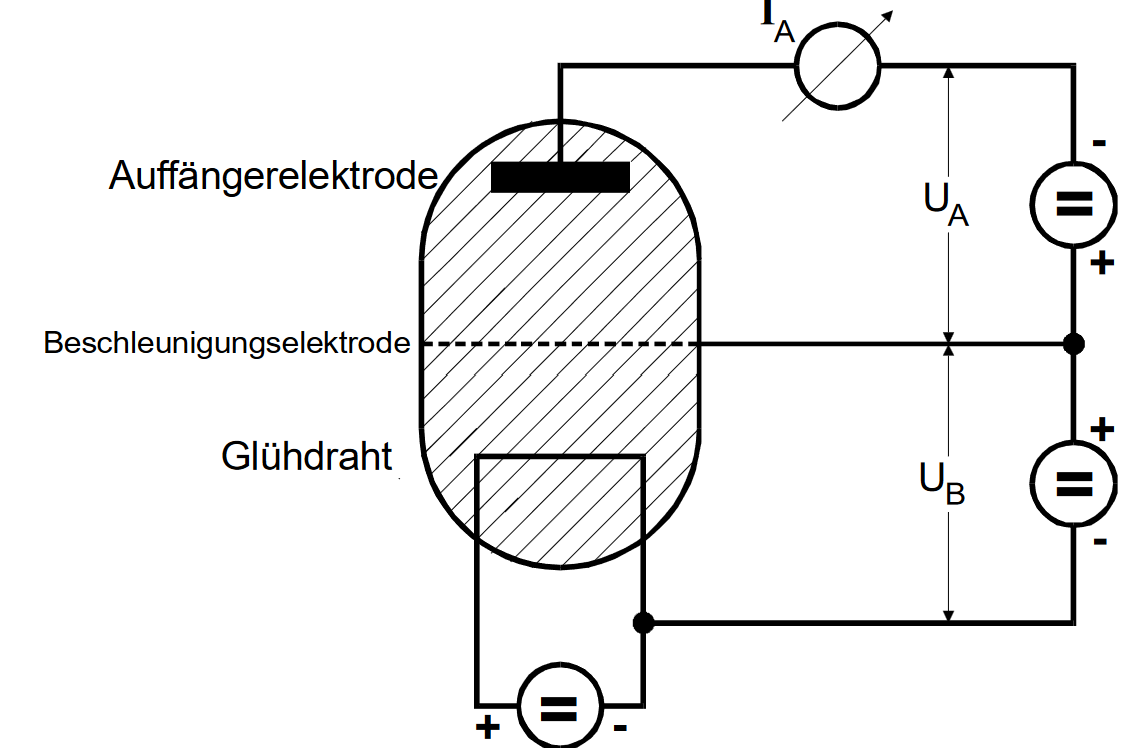
\includegraphics[width=0.75\linewidth]{content/grafik/aufbau.png}
	\caption{Der prinzipielle Aufbau des Frank-Hertz Versuches. \cite{franck}}
	\label{fig:aufbau}
\end{figure}

Die Appeartur des Franck-Hertz Versuches besthet aus einem evakuierten Gefäß, welches winzige Tropfen Quecksilber beinhaltet.
Das Quecksilber, verdampft gemäß der Dampfdruckkurve bis sich ein Gleichgewichtsdampfdruck $p_{\text{sät}}$ einstellt.Dieser ist von
der Umgebenungstemperatur $T$ abhängig, welche zur eingestellt werden kann, sodass die Dampfdichte reguliert werden kann. In den Glaskolben
wird ein Draht aus Wolfram eingeführt. An Diesen wird eine Heizspannung angelegt, sodass aufgrund des glühelektrischen Effekt
Elektronrn austreten. Gegenüber des Glühdrahtes befindet sich eine netzförmige Beschleunigungunselektrode an der eine Beschleunigungsspannung
$U_B$ angelegt ist, welche die Elekronen beschleunigt. Nach Durchlaufen der Beschleunigungsstrecke besitzen die Elektronen, welche
vorher eine Geschwindigkeit von $v = 0$ hatten, eine kinetische Energie mit 
\begin{equation*}
    \frac{m_0 \cdot v_{\text{vor}}^2}{2} = e_0 \cdot U_B.
\end{equation*}
$e_0$ entspricht dabei der Ladung eines Elektrons. Hinter der Beschleunigungunselektrode befindet sich eine Auffänerelektrode. 
In dem Zwischenraum beider Elekteoden wird ein Gegenfeld mit der Spannung $U_A$ angelegt. Somit wird die  Auffängerelektrode
ausschließlich von den Elektronen erreicht, welche die Bedingung
\begin{equation*}
    \frac{m_0}{2} v_Z^2 \,\geq\, e_0 U_A
\end{equation*}
erfüllen.

Es befinden sich Hg-Atome im Bescleunigungsraum, daher wechselwirken diese mit den Elektronen. dabei gibt es zwei Fälle von 
Wechselwirkung die auftreten können: Im ersten Fall ist die Elektronenenergie $E$ nicht hoch, so kommt es njur zu elastischen
Stößen. Aufgrund des Massenverhältnisses $m_0/M$ ergibt sich ein vernachlässigbarer Energieverlust
\begin{equation*}
    \increment E=\frac{4 \, m_{0} \, M}{\left(m_{0} + M\right)^{2}} \cdot E \approx \num{1.1e{-5}} \, E \, .
\end{equation*}
Wichtig zu beacten ist dabei, dass die Elektronen beträchtliche Richtungsänderungen erfahren.
Im zweiten Fall ist die Energie die Elektronen gleich oder größer der Energiedifferenz $E_1 - E_0$. Dan kommt es zu inelastischen
Stößen. Auf die Quecksilber-Atome wird der Betrag der Energiedifferenz übertragen, wodurch diese angeregt werden.
Daraufhin wird das Quecksilber-Atom unter Emission einer elektromagnetischen Welle wieder in den Grundzustand zurückgeführt.
Der Lichtquant besitzt dabei eine Energie von 
\begin{equation*}
    h v=E_1-E_0 ,
\end{equation*}
wobei h das Plancksche Wirkungsquantum und $\nu$ die Frequenz der emittierten Strahlung ist.

Um die Anregungsenergie der Hg-Atome zu bestimmen wird der Auffängerstrom $I_A$ in Abhängigkeit zur Beschleunigungsspanung $U_B$
betrachtet. Der idealisierte Verlauf ist in \autoref{fig:ideal} dargestellt.

\begin{figure}[H]
	\centering
	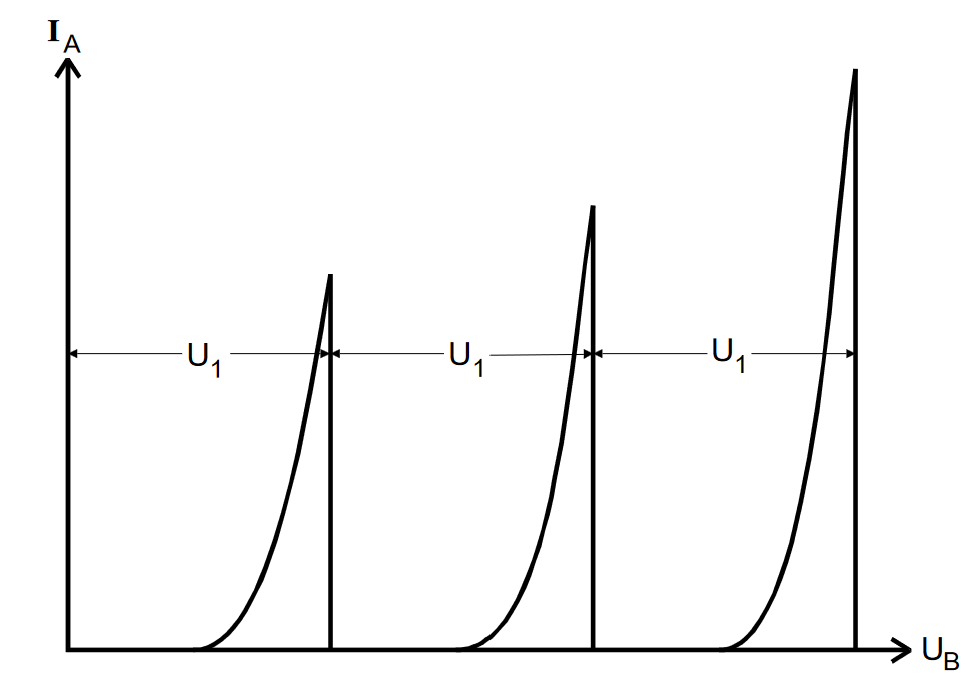
\includegraphics[width=0.75\linewidth]{content/grafik/idealisiert.png}
	\caption{Der idealisierte Verlauf des Auffängerstroms $I_A$ in Abhängigkeit zur Beschleunigungsspanung $U_B$. \cite{franck}}
	\label{fig:ideal}
\end{figure}

Es kann beobachtet werden, dass eine periodische Zu - und Abnahme des Anfängerstroms bei wachsender Beschleunigungsspanung
passiert. Wenn durch das Erhöhen von $U_B$ die Elektronenenergie $E_1 - E_0$ erreicht oder überragt, treten unelastische Stöße auf.
Dabei geben die Elektronen immer die Energiedifferenz $E_1 - E_0$ ab.
Der Abstand $U_1$ zweier aufeinader folgender Maxima muss dem 1.Anregungspotential entsprechen
\begin{equation}
    U_1:=\frac{\left(E_1-E_0\right)}{e_0} \, .
    \label{eqn:u1}
\end{equation}

Es gibt drei wichtige Nebeneffekte die beachtet werden müssen bei der realen Franck-Hertz Kurve. Diese sieht
nicht aus wie in \autoref{fig:ideal} gezeigt.

Das reale Beschleunigungspotential zwischen dem Glühdraht und der Beschleunigungselektrode ist von der außen
angelegten Spannung $U_B$ verschieden. Wenn beide Elketroden aus Materialien bestehen, die eine unterschiedliche
Austrittsarbeit für Elektronen besitzen. Es wird für den Glühdraht ein Material ausgewählt, dessen Austrittsarbeit  $\phi_G$
viel kleiner als die Austrittsarbeit $\phi_B$ der Beschleunigungselektrode ist. Das Potentialverhältnis ist
in \autoref{fig:potential} dargestellt.

\begin{figure}[H]
	\centering
	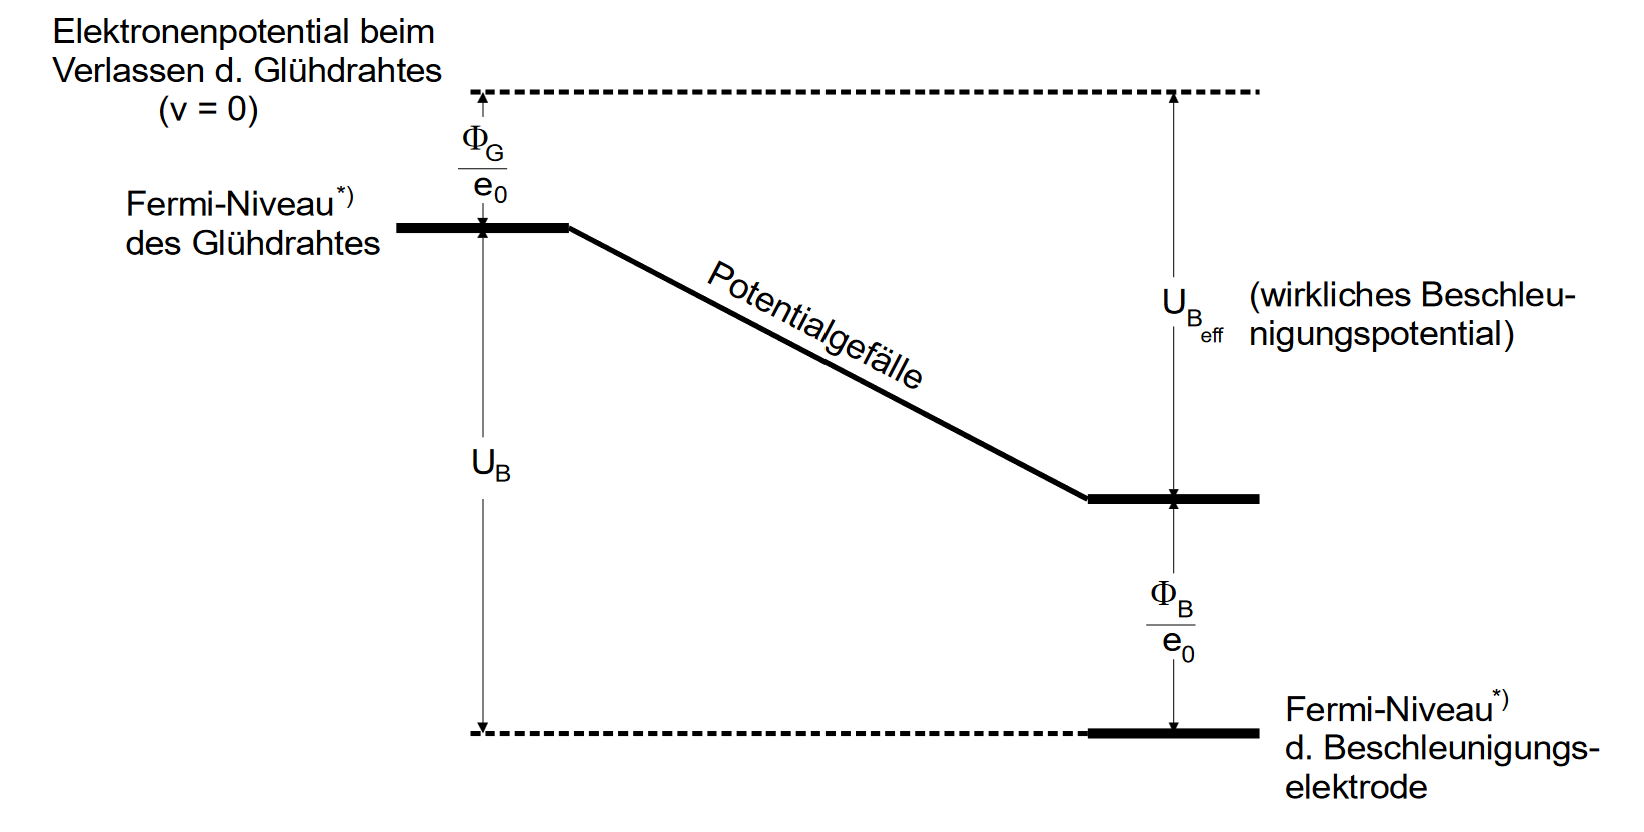
\includegraphics[width=1.0\linewidth]{content/grafik/potential.png}
	\caption{Potentialverhältnis zwiechen Glühkathode und Beschleunigungselektrode. \cite{franck}}
	\label{fig:potential}
\end{figure}

Für das eigentliche Beschleunigungspotential $U_{\text{B}, \text{eff}}$ gilt 
\begin{equation}
    U_{\text{B}, \text{eff}}=U_{\text{B}}-\frac{1}{e_0}\left(\phi_B-\phi_G\right).
    \label{eqn:potential}
\end{equation}
Der Ausdruck 
\begin{equation}
    K = \frac{\left( \phi_B - \phi_G \right)}{e_0} 
    \label{eq:Kontaktpotential} 
\end{equation}
entspricht dem Kontaktpotential. Die gemessene Franck-Hertz Kurve ist dabei um den Wert $K$ verschoben.

Zunächst wurde die Annahme getroffen,dass die Elekronen nach Durchlauf des Beschleunigungsraumes alle eine einheitliche 
Energie besitzen. Duese Annahme ist jedoch unzutreffend.Die Leitungselektronen besitzen in Inneren eines Metalles bereits 
ein Energie-Spektrum, welches als Fermi-Dirac-Verteilung bezeichnet wird.
Die unelastischen Stöße setzten bei einem sich erstreckten endlichen Einsatzbereich ein. Das führt dazu, dass
sich die Franck-Hertz Kurve in ihren Anstieg bei Annäherung an ein Maximum verringern und nicht mehr unstetig auf den Wert 0 abfallen.
Die Richtungsänderungen, die aufgrund von elastischen Stößen auftreten, führen zu keine merklichen Energieabnahmen der Elektronen.
Erst wenn diese Stöße zwischen Beschleunigungselektrode und Auffänerelektrode vorkommen, ensteht eine Verteilung
der z-Komponente der Geschwindigkeiten. Da das gegebene Gegenfeld eine $v_z$-Abhängigkeit vorweist, führen die elastischen
Stöße zu einer Abflachung und Verbreiterung der Franck-Hertz-Kurve.

Ebenfalls Einfluss auf den Verlauf der Franck-Hertz Kurve hat der Dampfdruck. Damit Zusammenstöße von Elektronen und Hg-Atomen 
auftreten können, muss die mittlere freie Weglänge $\bar{w}$ der Atome klein gegen den Abstande $a$ zwischen Kathode und Beschleunigungselektrode
sein. Die mittlere freie Weglänge $\bar{w}$ kann über den Sättigungsdampfdruck $p_{\text{sät}}$, der innerhalb der Röhre herrscht,
eingestellt werden. Aus der kinetischen Gastheorie geht hervor

\begin{equation}
    \bar{w} \, \left[\unit{\centi\meter}\right] = \frac{0.0029}{p_{\text{sät}}} \, \left[ \frac{1}{\unit{\milli\bar}}\right].
    \label{eqn:dampf1}
\end{equation}
Wenn der Dampfdruckbereich klein ist, kommt es auch bei gr0ßer Bremsspannung $U_B$ nur selten zu Anrgeungen, wobei bei einem 
sehr hohen Dampfdruckbereich der Energieverlust der elastischen Stöße wichtig ist, da oft zu Zusammenstößen kommt.
Die Dampfdruckkurve wird gemäß
\begin{equation}
    p_{\text{sät}} (T) = \num{5.5e7} \exp{\left( \frac{-6876}{T} \right)} 
    \label{eqn:dampf2}
\end{equation}
berechnet.